\chapter{Architettura del sistema}
\label{capitolo3}
\thispagestyle{empty}

\noindent In questo capitolo si descriverà la progettazione del sistema creato. Inizialmente si tratterà l'analisi del progetto e le scelte effettuate per quanto riguarda gli strumenti da utilizzare. Successivamente si descriveranno tutti i moduli che compongono l'architettura del sistema. La trattazione è divisa in parte hardware e parte software.
\section{Analisi del sistema hardware}
L'obiettivo del progetto è quello di creare uno strumento che permetta all'utilizzatore di pedalare, sterzare e osservare un luogo in un mondo virtuale. In primo luogo, era necessario creare un sistema simile ad una bicicletta. Ai fini di sperimentazione della tipologia di progetto, si è scelto di utilizzare una cyclette. La suddetta, permette di semplificare notevolmente il sistema elettronico e il sistema software, poiché questi non devono tenere conto dell'attrito e del ritorno di forza, in quanto una pedalata farà sempre ruotare il volano. La cyclette è inoltre sprovvista di freni, i quali potrebbero essere utilizzati per frenare la bicicletta virtuale. Si è quindi scelto di ottenere solo le informazioni relative alla pedalata e alla posizione del manubrio. Queste informazioni devono essere elaborate da un microcontrollore che ottiene i dati da tutti i sensori e genera una macro-informazione da inviare al sistema software.

\subsection{Sensori del manubrio}
\begin{figure}%
    \centering
    \subfloat[I 4 fotodiodi]{{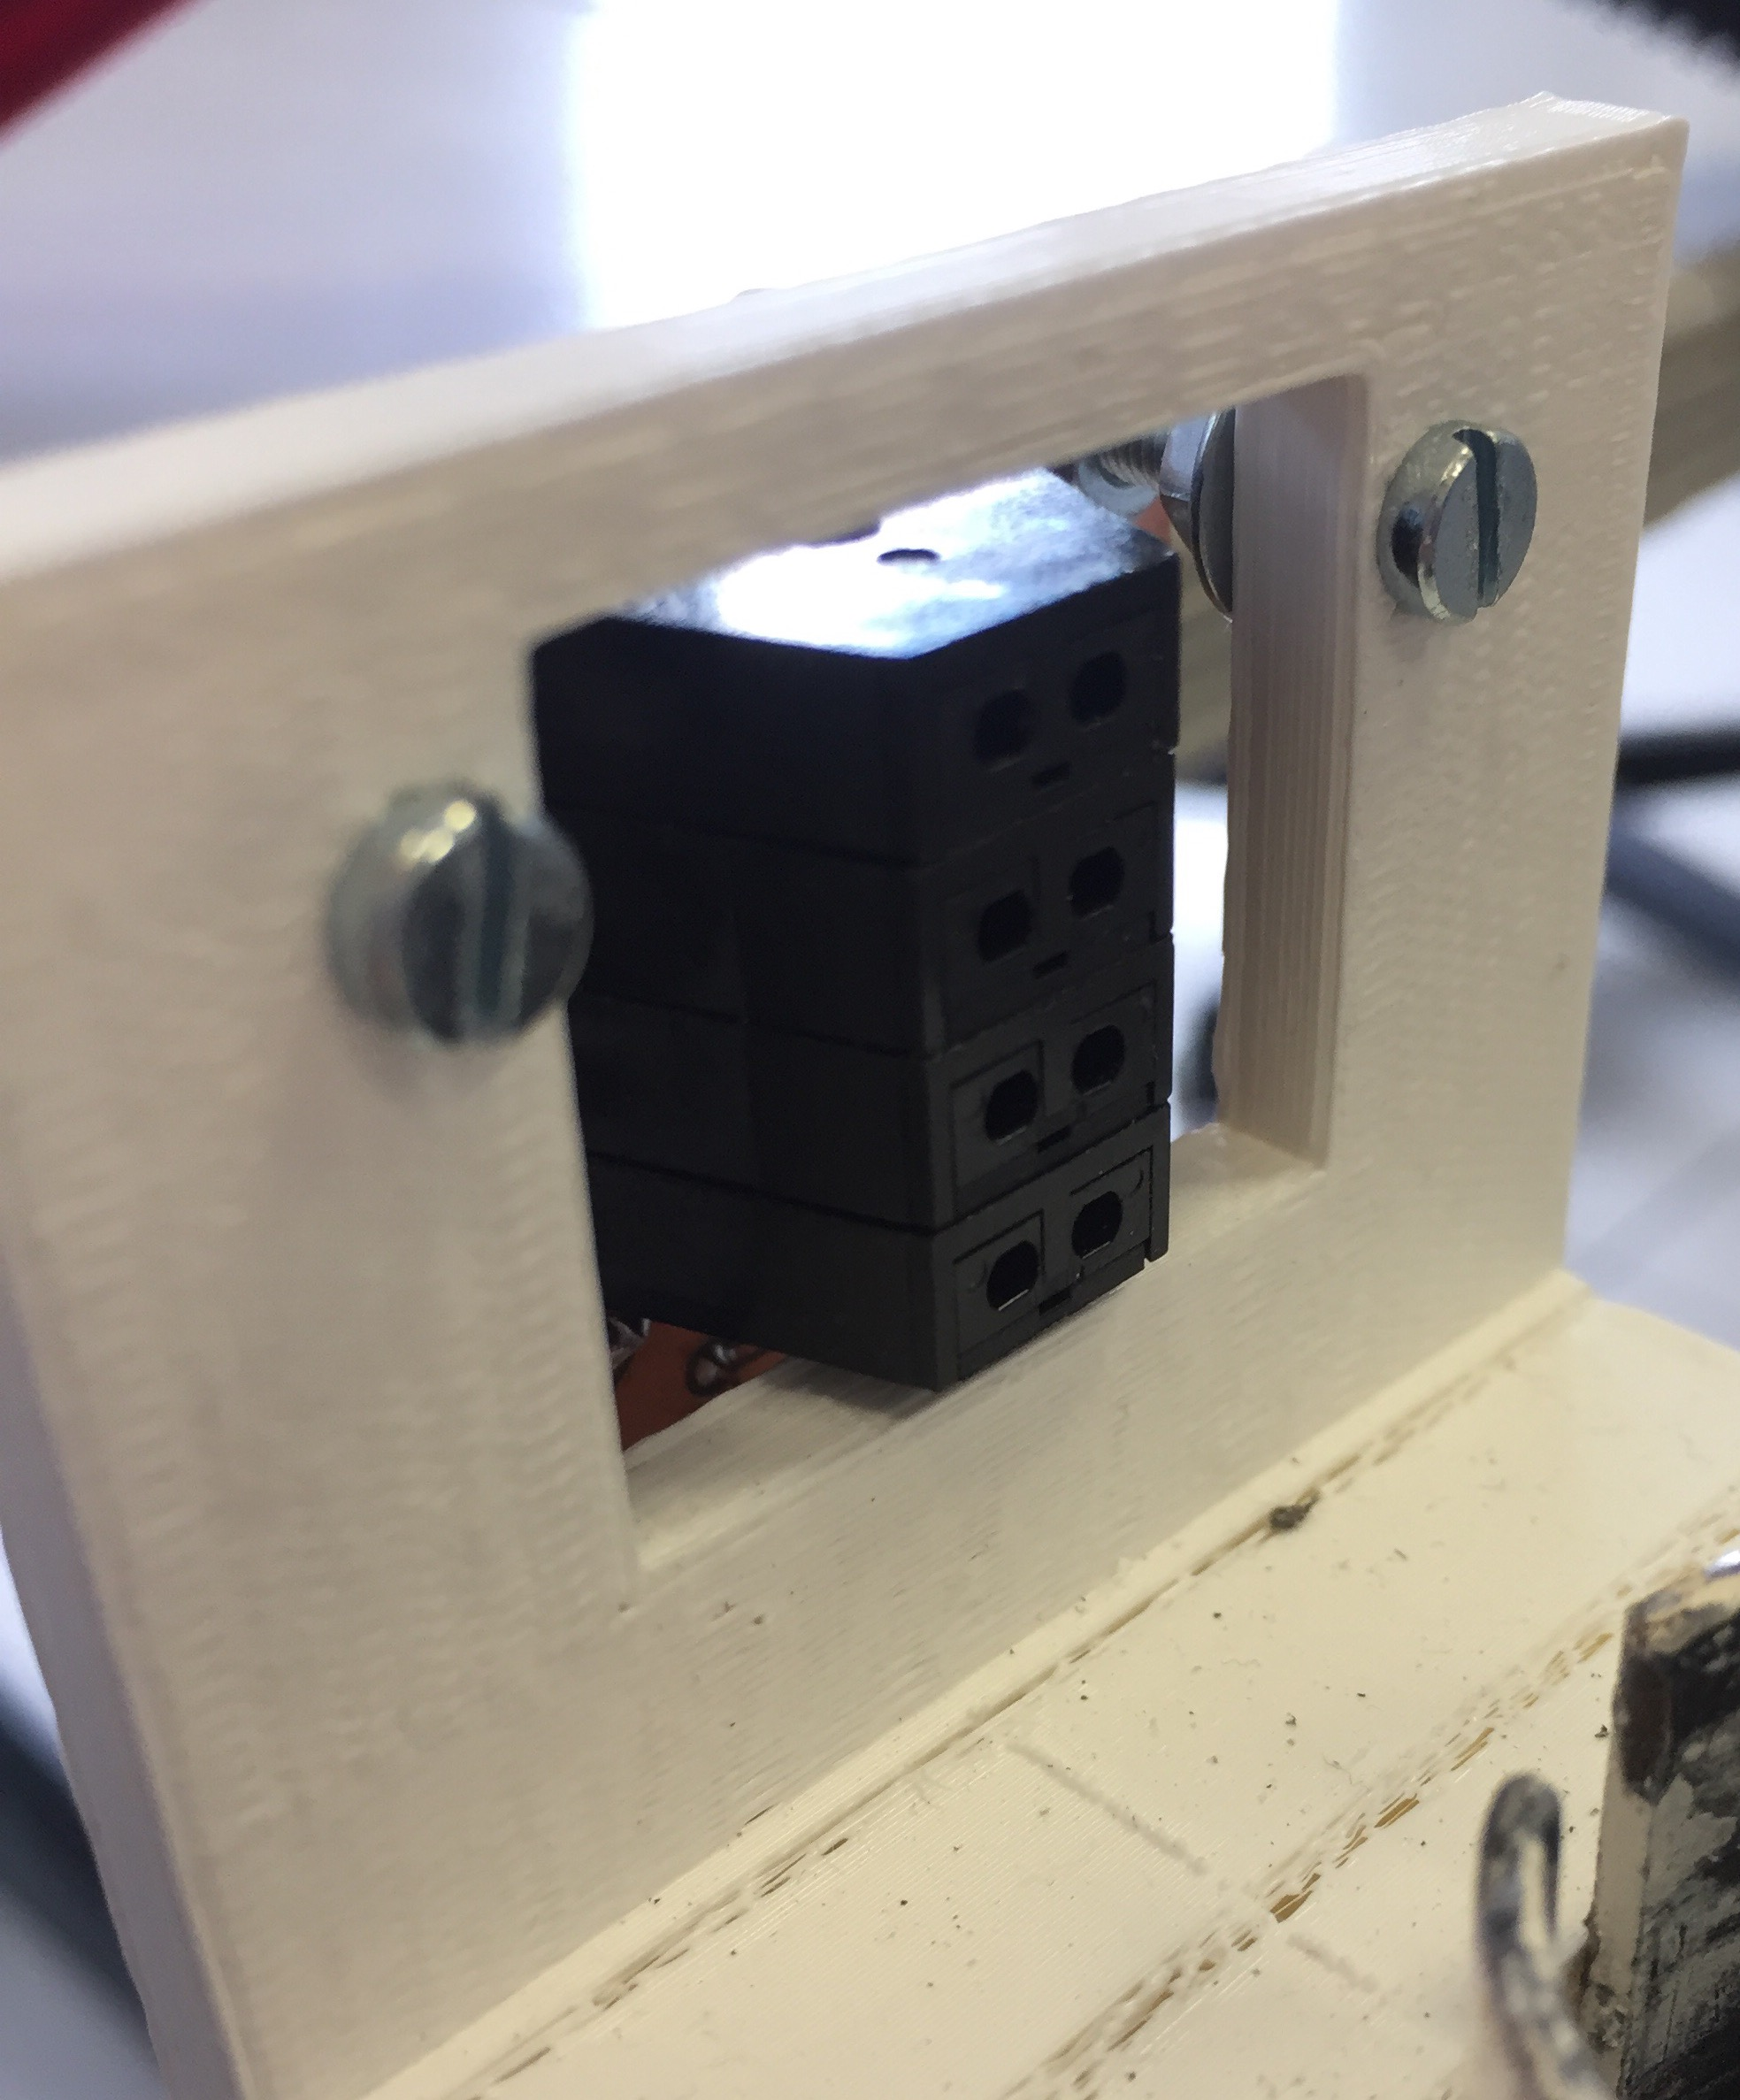
\includegraphics[height=5.5cm]{4Fotodiodi} }}%
    \subfloat[Le 16 posizioni in permutazione ciclica]{{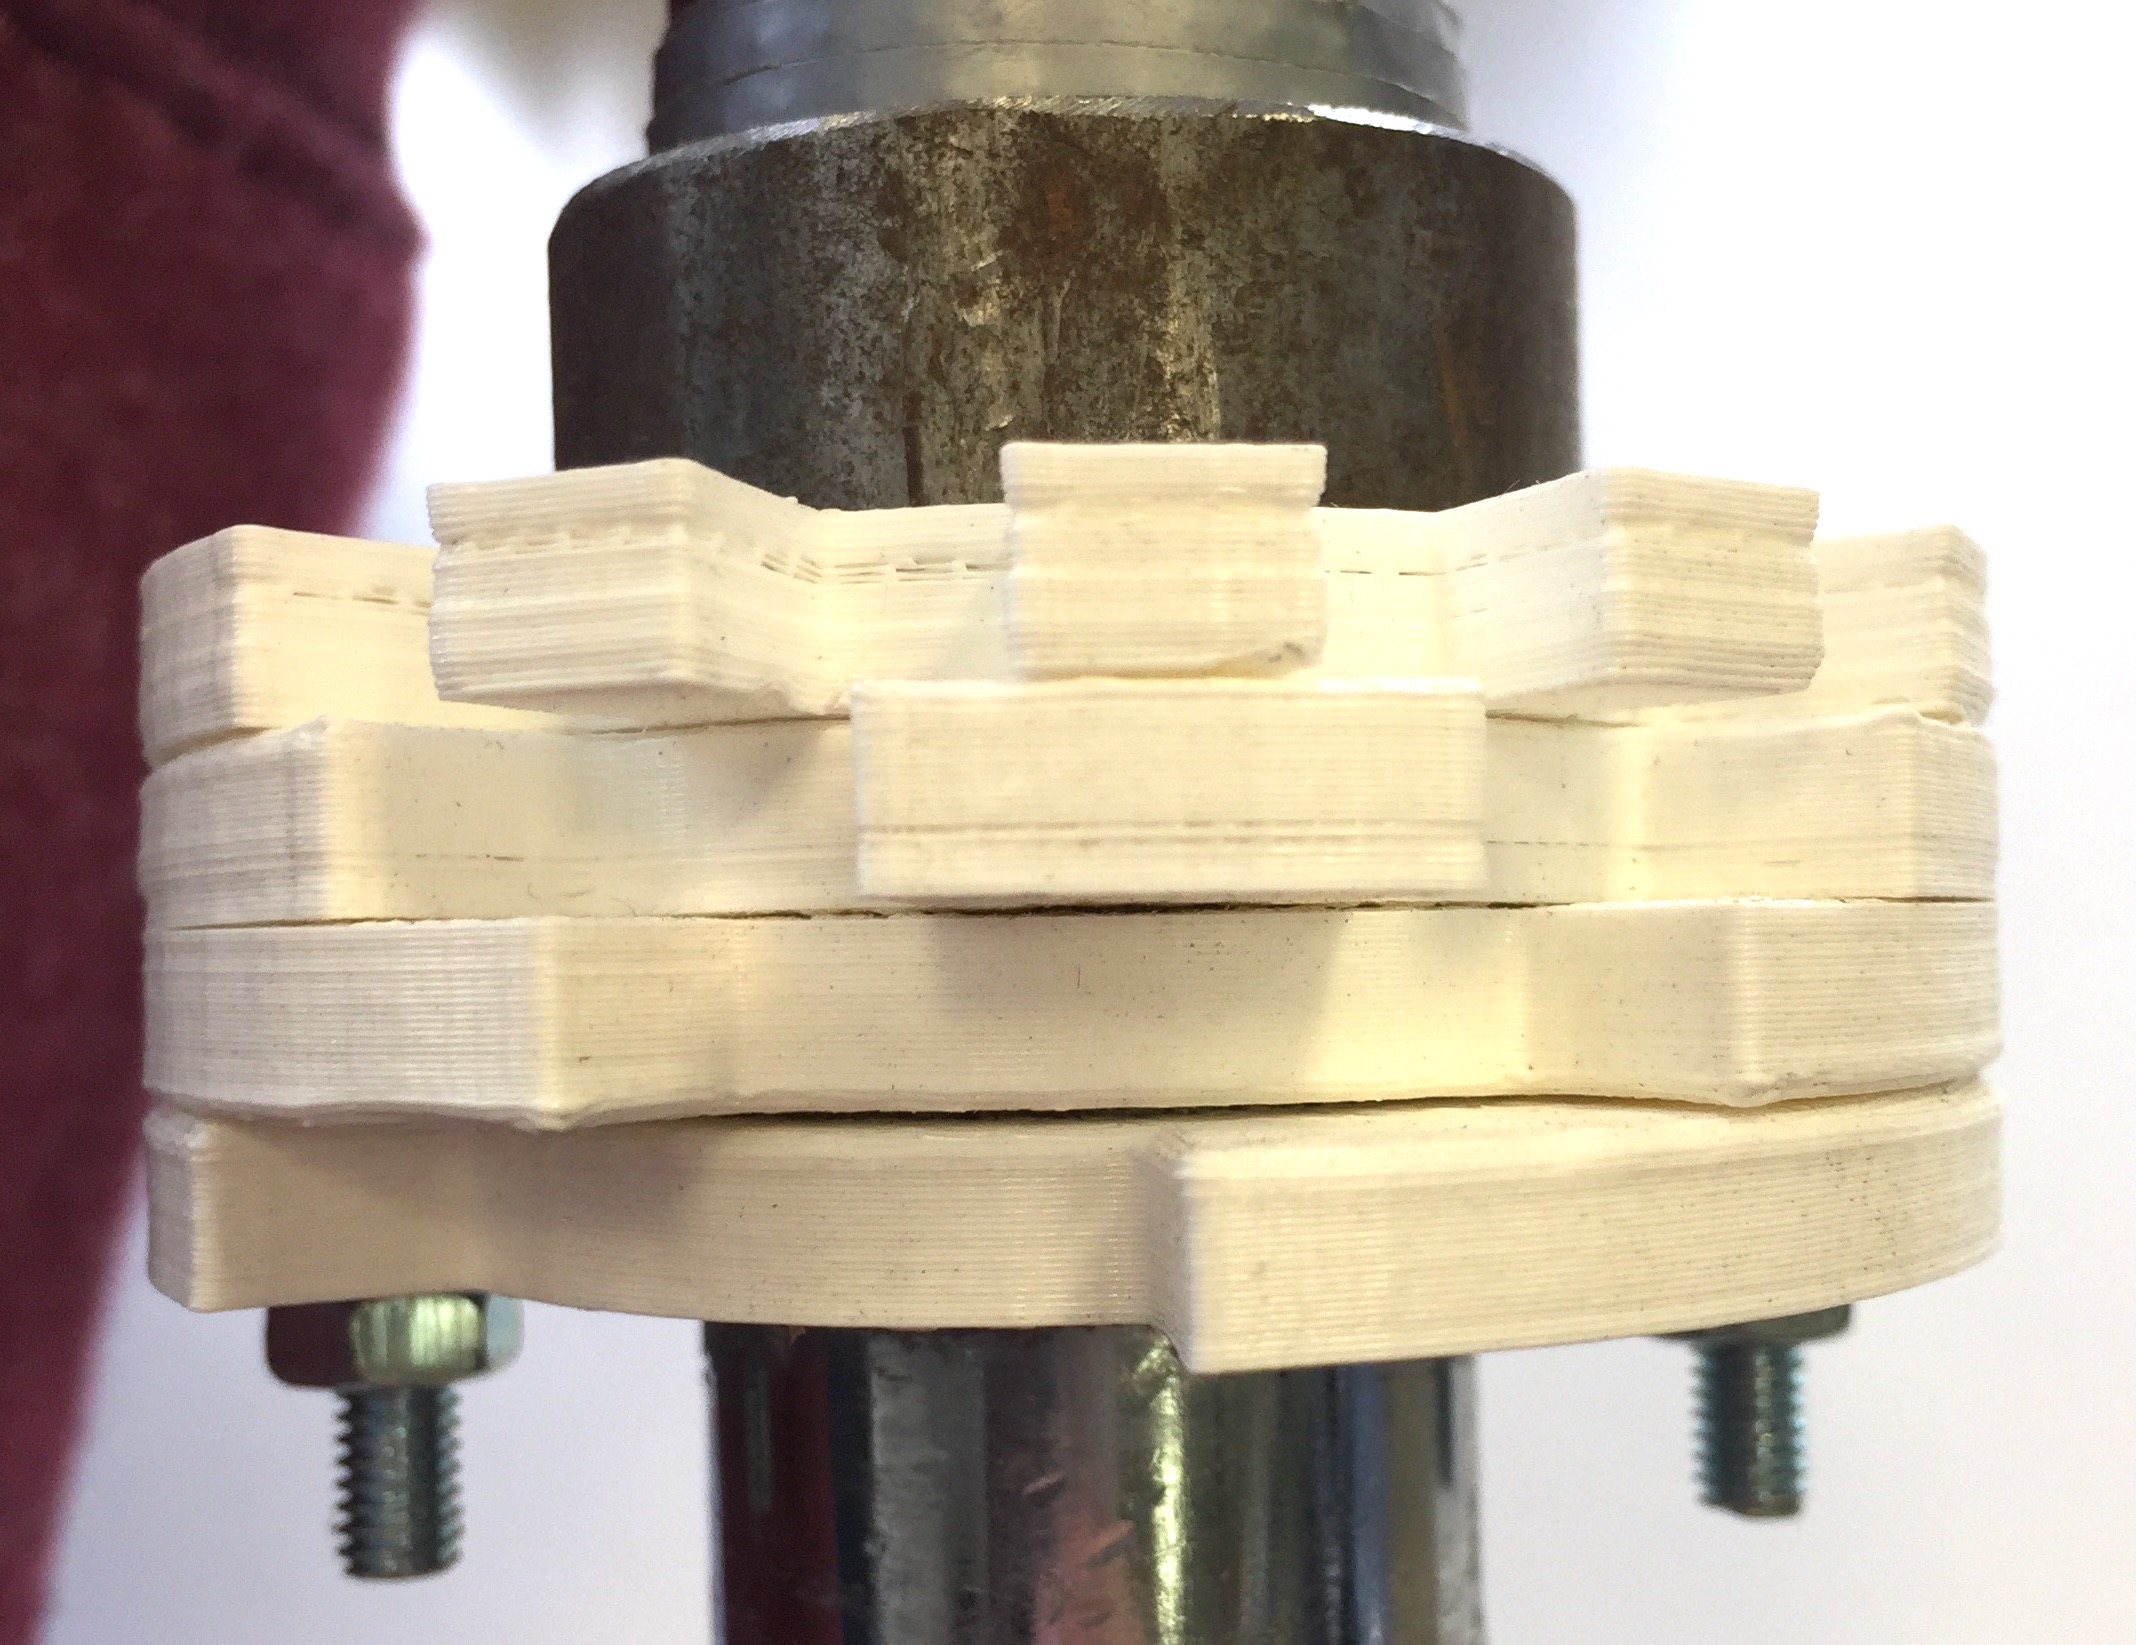
\includegraphics[height=5.5cm]{codifica4bitManubrio} }}%
    \caption{Sensori del manubrio}%
    \label{manubrio}
\end{figure}
Per ottenere le informazioni relative alla posizione del manubrio è stato scelto un angolo massimo di rotazione di 120\degree. Questo angolo è stato diviso in 16 posizioni. \\
\begin{wrapfigure}{r}{0.2\textwidth} %this figure will be at the right
    \centering
    \vspace{-1.5cm}
    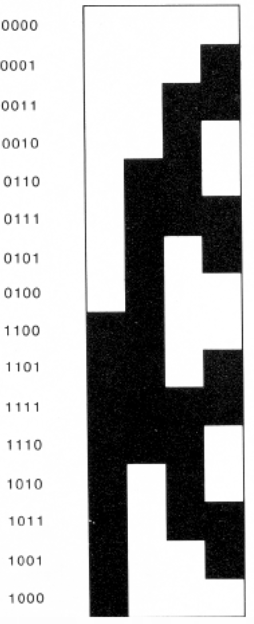
\includegraphics[width=0.2\textwidth]{codifica4bit}
\end{wrapfigure}
Per poter rilevare la posizione corrente è stata necessaria una codifica in 4 bit. Per ottenere questa codifica, si è fatto uso di 4 fotodiodi\footnote{Il fotodiodo è un particolare tipo di diodo fotorilevatore che funziona come sensore ottico sfruttando l'effetto fotovoltaico, in grado cioè di riconoscere una determinata lunghezza d'onda dell'onda elettromagnetica incidente (assorbimento del fotone) e di trasformare questo evento in un segnale elettrico di corrente applicando ai suoi estremi un opportuno potenziale elettrico. Esso è dunque un trasduttore da un segnale ottico ad un segnale elettrico.} che permettono di rilevare i 4 spazi che compongono una delle delle 16 configurazioni. I fotodiodi permettono di distinguere uno spazio vuoto da uno spazio pieno creando un segnale elettrico. Le configurazioni sono state realizzate con un oggetto stampato con stampante 3D, come si vede in figura \ref{manubrio}b, in permutazione ciclica (figura a lato), che permette di accorpare gli \textit{uni} e gli \textit{zeri} e ridurre l'alternanza di \textit{vuoti} e \textit{pieni}.


\subsection{Sensori del volano}
\begin{wrapfigure}{l}{0.4\textwidth} %this figure will be at the right
    \centering
    \vspace{-0.3cm}
    
\includegraphics[height=5.5cm]{placeholder}
    \caption{Il volano della cyclette e l'accelerometro}
    \vspace{-1cm}
\end{wrapfigure}
La bicicletta virtuale deve muoversi ad una velocità consona alla rotazione del volano della cyclette. Quest'ultimo è stato quindi munito di un accelerometro che fornisce informazioni sulla velocità di rotazione. Sui pedali sono stati inoltre installati due fotodiodi che permettono distinguere se la rotazione è oraria o antioraria. La direzione di rotazione viene ottenuta distinguendo quale dei due fotodiodi viene oscurato per primo. Ad esempio, se consideriamo due fotodiodi disposti orizzontalmente:\\
%=========aggiungi immagini e riferimento a immagini
\begin{itemize}
  \item Se un oggetto passa da sinistra a destra, si oscurerà prima il fotodiodo sinistro poi il destro, quindi assumendo un oggetto che abbia il fulcro di rotazione sotto i fottodiodi, la sua rotazione è \textbf{oraria}
  \item in caso contrario, la rotazione è \textbf{antioraria}.
\end{itemize}

\subsection{Microcontrollore}
\begin{wrapfigure}{r}{0.4\textwidth} %this figure will be at the right
    \centering
    \vspace{-1.3cm}
    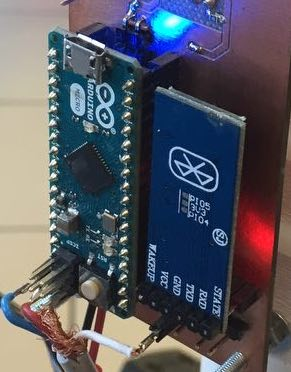
\includegraphics[height=5.5cm]{arduino}
    \caption{La scheda Arduino Micro e il modulo bluetooth}
    \vspace{-1.3cm}
\end{wrapfigure}

%=========CHIEDI a lanzoni come viene ottenuto il dato dall'accelerometro e come viene ottenuto il + e il -
Il cuore della parte hardware è la scheda Arduino che elabora tutti i dati ricevuti via cavo o via bluetooth. La scheda con il microcontrollore è in continua comunicazione in input e in output con il modulo bluetooth poiché deve ricevere l'informazione sulla rotazione dall'accelerometro e deve inviare all'elaboratore esterno una stringa contenente tutte le informazioni sotto forma di stringa.
\subsubsection{Stringa}
La stringa elaborata dall'Arduino è composta come segue:
\begin{itemize}
  \item \textbf{Posizione del manubrio}: un valore compreso tra 0 e 15 che indica la posizione del manubrio
  \item \textbf{Velocità di rotazione}: un valore compreso tra 0 e 40 che indica la velocità di rotazione della pedalata.
  \item \textbf{Senso di rotazione}: un segno \textbf{+} o \textbf{-} che indica senso orario o antiorario di rotazione della pedalata.
\end{itemize}

\noindent Un esempio pratico è \textbf{12+27.5}: significa che si sta registrando una pedalata in senso orario con velocità 27.5 e il manubrio è nella posizione 12.

\subsection{Ricevitore Bluetooth}
La ricezione della stringa avviene tramite un ricevitore bluetooth collegato ad una porta USB del computer generale in cui viene eseguito il software. Utilizzando un programma terminale apposito, chiamato HyperTerminal è stato possibile leggere la porta seriale COM a cui vengono inviati i dati a 9600 bit/s e testare la parte hardware.
\subsection{OSVR}
\begin{figure}[htb]
    \centering
    \vspace{-0.7cm}
    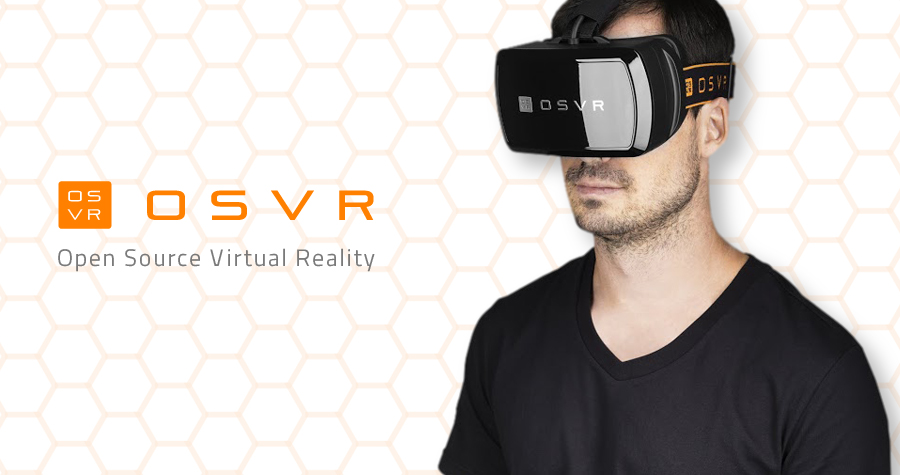
\includegraphics[width=\textwidth]{osvr1}
    \vspace{-0.3cm}
\end{figure}
\noindent OSVR é l'acronimo di \textit{Open-Source Virtual Reality} ed identifica la piattaforma software open-source per la Realtà Virtuale e quella aumentata. \\È stata sviluppata dalla Razer e da Sensics. La prima è l'azienda leader nel settore del gaming, mentre la seconda lo è nel settore della realtà virtuale. Affinché questa piattaforma sfondasse nel mercato, le società sopracitate hanno deciso di rendere open-source sia il software sia l'hardware per i programmatori. È infatti reperibile su github il codice sorgente. OSVR consente in modo davvero semplice la configurazione e la gestione dei vari dispositivi: occhiali VR, inseguitori di posizione, periferiche di gioco e vari altri. 
\subsubsection{Caratteristiche}

\begin{wrapfigure}{r}{0.5\textwidth} %this figure will be at the right
    \centering
    \vspace{-0.5cm}
    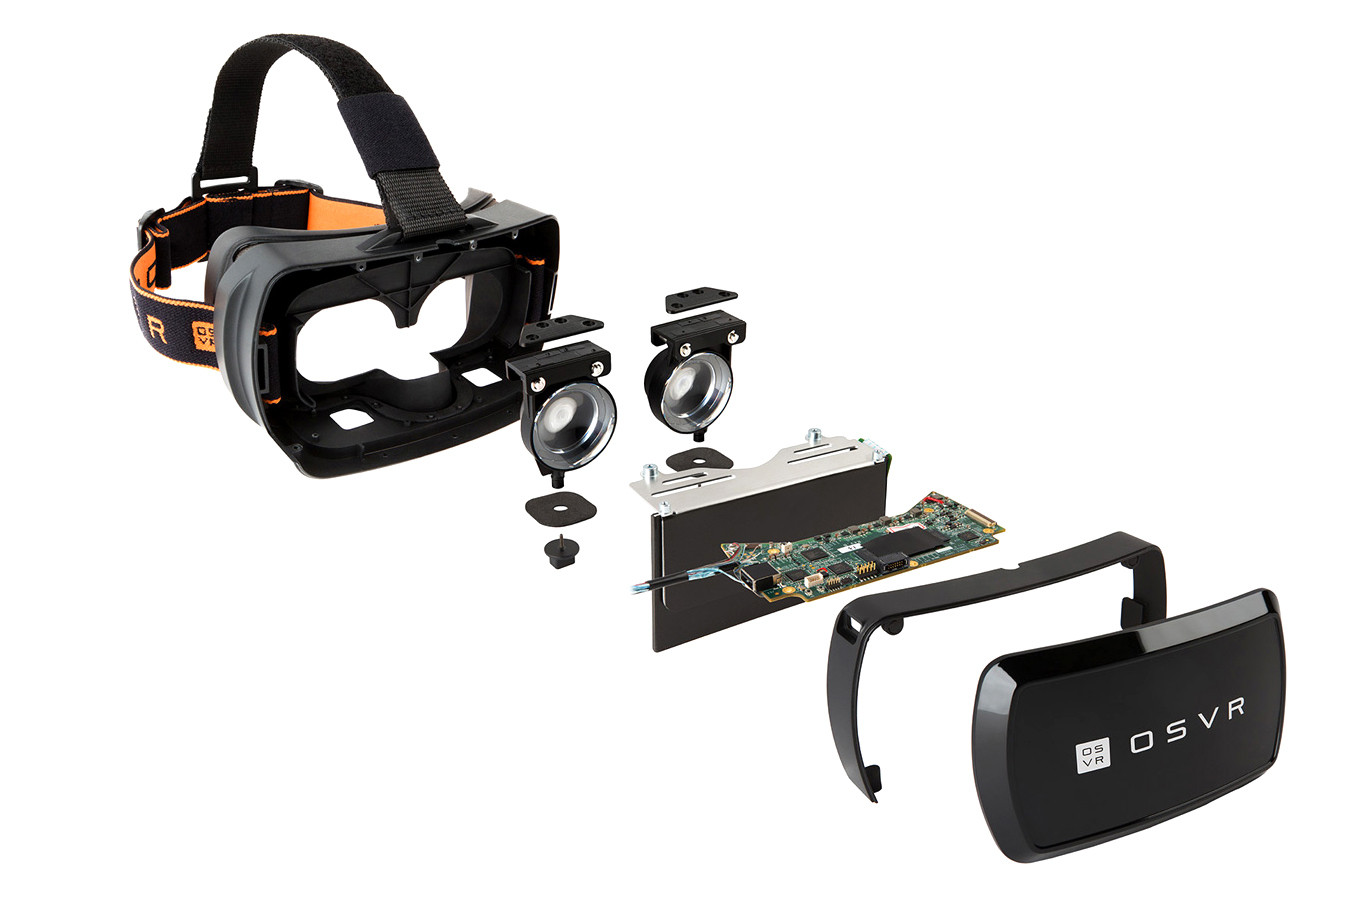
\includegraphics[width=7cm]{osvr2}
    \caption{I componenti del visore OSVR HDK1}
    \vspace{-0.3cm}
\end{wrapfigure}
L'OSVR è composto da un display montato su una visiera, o meglio head-mounted (HMD), da 2 lenti amovibili, da un display OLED da 5.5 pollici con risoluzione 1920 x 1080 pixel, 60 fps di refresh rate e campo visivo di 100 gradi. Contiene una scheda madre riprogrammabile con accelerometro e giroscopio integrati. Il visore OSVR dispone di doppie lenti che consentono di ridurre la distorsione delle immagini. A differenza di altri visori, questo dispone di una cintura elastica che porta i cavi fino all'altezza del muscolo trapezio dell'utilizzatore, in modo da non limitarne il movimento e quindi l'esperienza di gioco.
Il punto forza di questa piattaforma è la facile integrazione con dispositivi e con software aggiuntivi. Ad esempio, utilizzando una telecamera eye-tracking è possibile adoperare il software fornito dal produttore della fotocamera per calcolare la direzione dello sguardo. È inoltre possibile utilizzare il visore in praticamente il 90\% dei sistemi operativi.
In questo modo lo sviluppatore non ha più bisogno di scegliere anticipatamente un particolare sistema operativo per la sua applicazione, la cui realizzazione richiederà meno tempo sfruttando i plug-in dei quali l'OSVR dispone. Si permette così allo sviluppatore di concentrarsi su essa piuttosto che sull'interfacciamento.
 Sono inoltre reperibili all'interno di Github, tutti i plug-in di integrazione con i vari motori grafici quali Unity e Unreal Engine.
\subsubsection{Integrazione}
L'integrazione dell'OSVR verrà trattata nella sezione \textit{\nameref{software}} in cui si descriverà il procedimento per installare, configurare ed utilizzare il visore.

%============PARTE SOFTWARE=============%
\section{Analisi della Parte Software}
\label{software}
La parte software è stata scritta interamente nel linguaggio \Csharp\: e si avvale del motore grafico Unity. L'applicazione crea un'ambientazione virtuale in cui viene posizionata una bicicletta a cui viene collegato uno script che legge continuamente la porta COM su cui il microcontrollore invia la stringa contente l'informazione di movimento. Lo script parsifica la stringa e dà i valori in pasto al motore grafico che muove la bicicletta virtuale.
\subsection{Blender}
\begin{wrapfigure}{r}{0.2\textwidth} %this figure will be at the right
    \centering
    \vspace{-1.0cm}
    
\includegraphics[height=2cm]{blender}
\end{wrapfigure}
Blender è un software libero e multipiattaforma di modellazione, animazione, compositing e rendering di immagini tridimensionali. Inoltre dispone di funzionalità per mappature UV e simulazioni di rivestimenti adatte alla creazione di applicazioni e giochi 3D. All'interno di Blender tutte le funzioni e le interfacce possono essere richiamate con scorciatoie e per questo motivo quasi tutti i tasti sono collegati a numerosi comandi. La sua interfaccia si basa essenzialmente sulla finestra principale di lavoro, in cui è possibile visualizzare un modello 3D e modificarlo. 
\begin{figure}[hbt]
\centering
  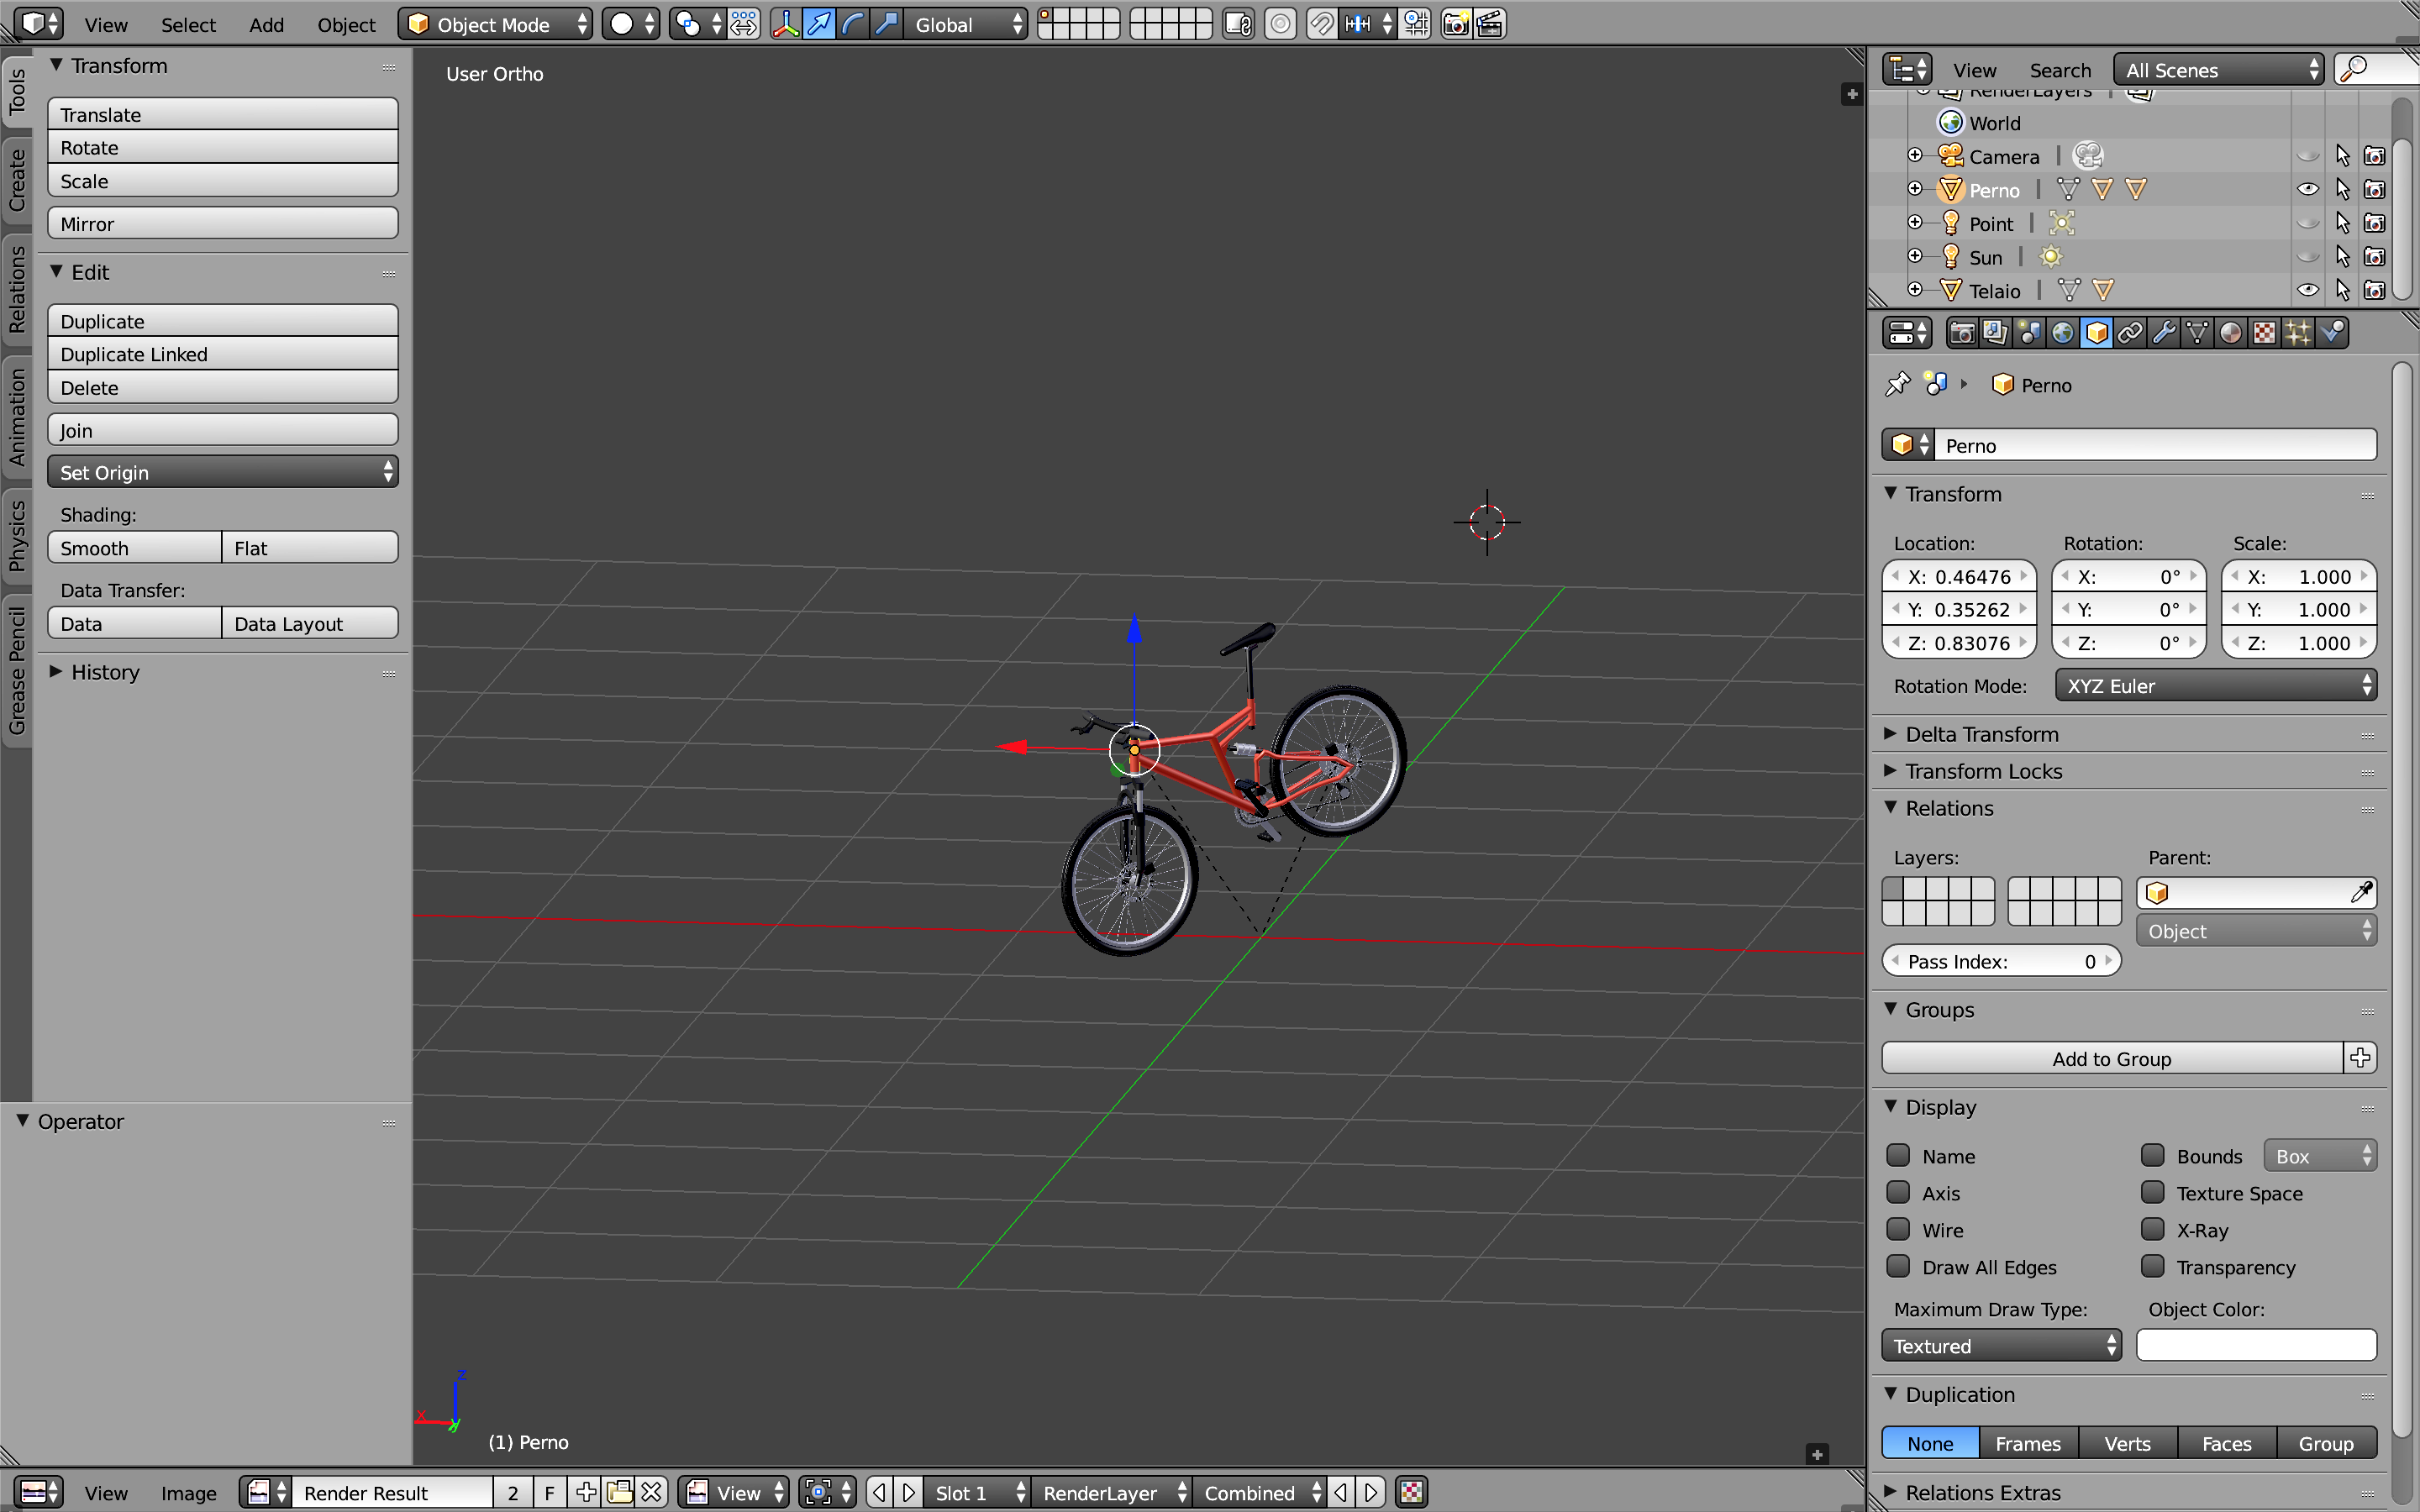
\includegraphics[height=8cm]{schermoblender.png}
  \caption{Interfaccia Principale di Blender}
\end{figure}

\noindent L'\textit{Object Mode} è la modalità che permette di visualizzare le mesh\footnote{Una mesh poligonale, anche detta maglia poligonale, è una collezione di vertici, spigoli e facce che definiscono la forma di un oggetto poliedrico nella computer grafica 3D e nella modellazione solida.} dell'oggetto, mentre l'\textit{Edit Mode} permette di modificarlo. Vi sono altre modalità che non sono state utilizzate, ma risultano utili per una modellazione più dettagliata. Per dotare il modello di texture o di materiali, ovvero l'applicazione di colori, trasparenza, lucentezza o altro, Blender implementa diverse finestre come la \textit{UV/Image Editor} nella quale è possibile scegliere la texture da applicare all'oggetto. Blender è stato utilizzato per creare la mesh della bicicletta virtuale da manovrare attraverso script collegati ad un motore grafico.
\subsubsection{Mesh della bicicletta}
%\begin{wrapfigure}{l}{0.5\textwidth} %this figure will be at the left
%    \centering
%    \vspace{-0.5cm}
%    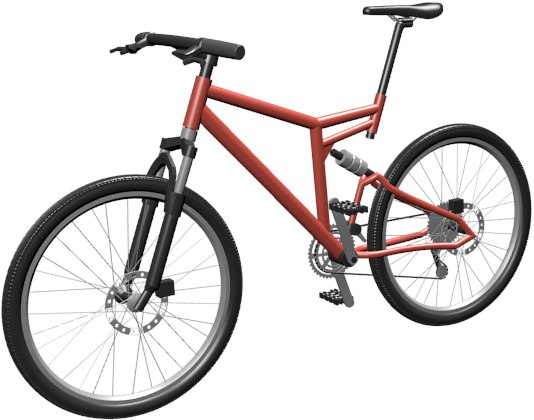
\includegraphics[height=5cm]{meshbici}
%\end{wrapfigure}
 \begin{figure}[htb]
    \centering
    %\vspace{-0.7cm}
    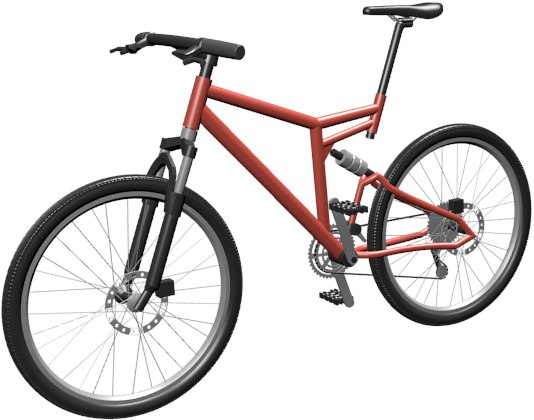
\includegraphics[height=8cm]{meshbici}
%    \caption{\label{fig:meshbici}}
    %\vspace{-0.3cm}
\end{figure}
\noindent La mesh proviene dal sito TurboSquid. È stata scaricata gratuitamente con estensione FBX\footnote{FBX è un formato di file di Autodesk che viene supportato dai più comuni software di grafica 3D in quanto è in grado di immagazzinare non solo geometrie, ma anche dati di texture e di animazioni.} ed è stata adattata per l'utilizzo necessario ai fini del progetto. È stata ridotta in scala ed è stata centrata alle coordinate (0,0,0). La mesh scaricata era già suddivisa in tutti i componenti di una bicicletta classica. Le uniche parti che devono essere dissociate ai fini della tesi sono il manubrio e il telaio. Sono state quindi assemblate tutte le mesh che compongono il telaio e tutte quelle che compongono il manubrio. Blender permette di associare un centro ad ogni mesh con la funzione \texttt{Set Origin > Origin to Geometry}. Questa permette di fornire, a tempo di esecuzione, una rotazione attorno al centro così definito. Sono state quindi lasciate libere le ruote e sono state centrate nel loro origine, in modo da poter dare una rotazione attorno al proprio asse.
\noindent La mesh della bicicletta è stata quindi suddivisa come segue:
\begin{itemize}
  \item \textbf{Telaio}: comprende tutto il telaio della bicicletta escluso il manubrio e le ruote.
	\begin{itemize}
  \item \textbf{Ruota posteriore}: è stata separata per darle possibilità di ruotare sul suo asse.
 \end{itemize}
  \item \textbf{Perno}: consiste nell'unione tra ruota e manubrio. Questo oggetto permette di ruotare tutto il manubrio mantenendo però un asse di rotazione inclinato. Comprende:
 \begin{itemize}
 \item \textbf{Manubrio}: contiene il manubrio stesso, la forcella e l'asse di sterzo.
 \item \textbf{Ruota anteriore}: è stata separata per darle la possibilità di ruotare sul suo asse.
 \end{itemize}
\end{itemize}

\begin{wrapfigure}{r}{0.35\textwidth} %this figure will be at the right
    \centering
    \vspace{-1.3cm}
    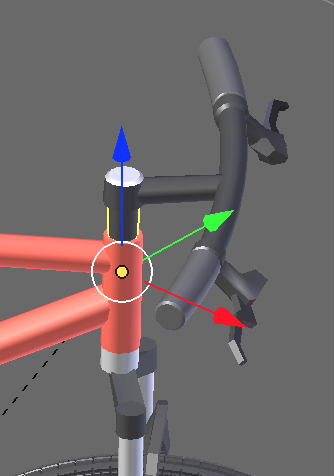
\includegraphics[height=5.5cm]{assebici}
    \caption{L'asse del canotto della bicicletta}
    \vspace{-1.3cm}
\end{wrapfigure}
\noindent Il telaio è stato separato dal manubrio solo nell'asse di sterzo, ma è stato mantenuto il canotto di sterzo, in modo da poter ruotare il manubrio attorno all'asse passante per il centro del canotto. La mesh così ottenuta è stata esportata ed è stata importata in Unity come oggetto da manovrare tramite script.\\
\subsubsection{Mesh dell'ambientazione}
L'ambientazione è stata fornita dal Cineca: si tratta di un modello 3D dei portici di San Luca (Bologna) ottenuto tramite rilevazione laser. Il modello riporta fedelmente tutti i dettagli spaziali dei portici, ma non riportano la texture. Per il progetto che è stato creato, l'ambientazione non ha alcuna rilevanza: è possibile asportare la bicicletta e posizionarla in un qualsiasi altro mondo virtuale, purché sia adatto al movimento di una bicicletta al suo interno. L'ambientazione può essere munita di luce principale sia su blender che sul motore grafico. L'importante è non sovrapporre troppo luci per non rischiare la sovra esposizione. In figura \ref{fig:portici} possiamo notare il modello dei portici in un'ambientazione vuota.
	\newpage
\begin{figure}[htb]
    \centering
    \vspace{-0.7cm}
    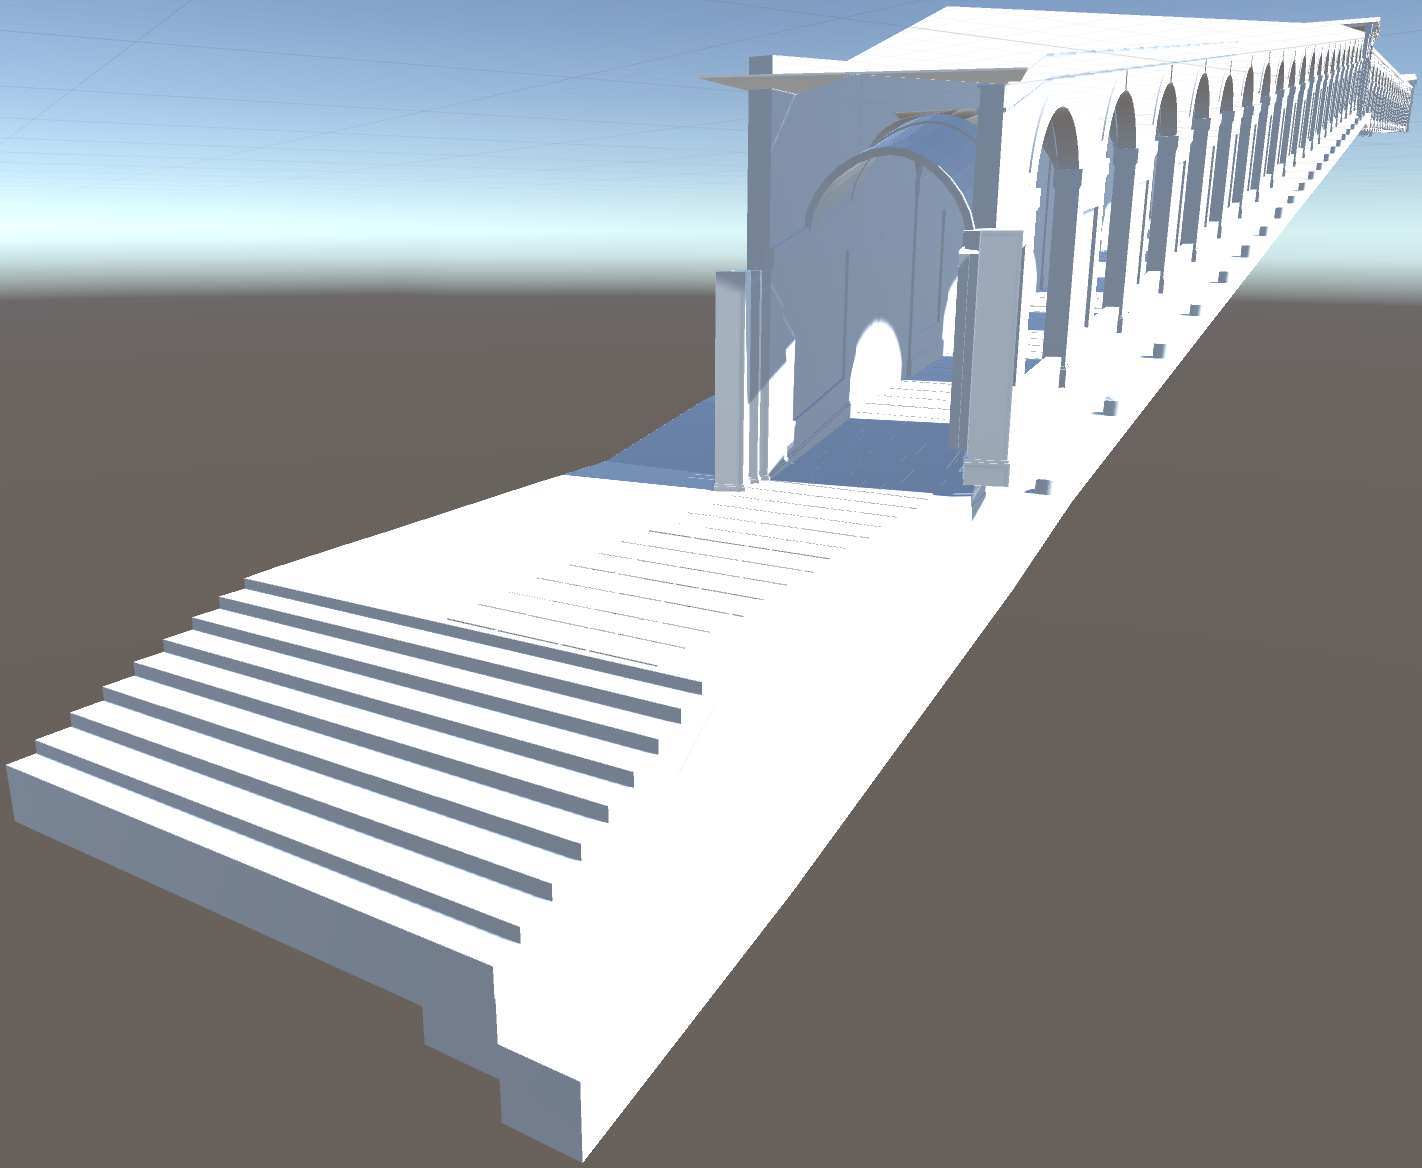
\includegraphics[width=\textwidth]{portici}
    \caption{Il modello dei portici di San Luca\label{fig:portici}}
    \vspace{-0.3cm}
\end{figure}

\subsection{Unity}
\noindent 
\begin{wrapfigure}{r}{0.2\textwidth} %this figure will be at the right
    \centering
    \vspace{-1.3cm}
    
\includegraphics[height=3cm]{unityicon}
    \vspace{-1.3cm}
\end{wrapfigure}
Unity è un motore grafico integrato multipiattaforma per la creazione di videogiochi o altri contenuti interattivi 3D, quali visualizzazioni architettoniche o animazioni 3D in tempo reale. Unity permette di modellare l'ambientazione 3D e il modello della bicicletta virtuale attraverso script. Permette inoltre di integrare il visore per la Realtà Virtuale ed è per questo che la scelta è ricaduta su questo motore grafico: per via della facile integrazione dei visori quali OSVR e Oculus Rift. 

\subsubsection{Schermata Principale} 
La schermata principale di figura \nameref{fig:screenunity} si compone di 5 riquadri suddivisi in:
 \begin{figure}[htb]
    \centering
    \vspace{-0.7cm}
    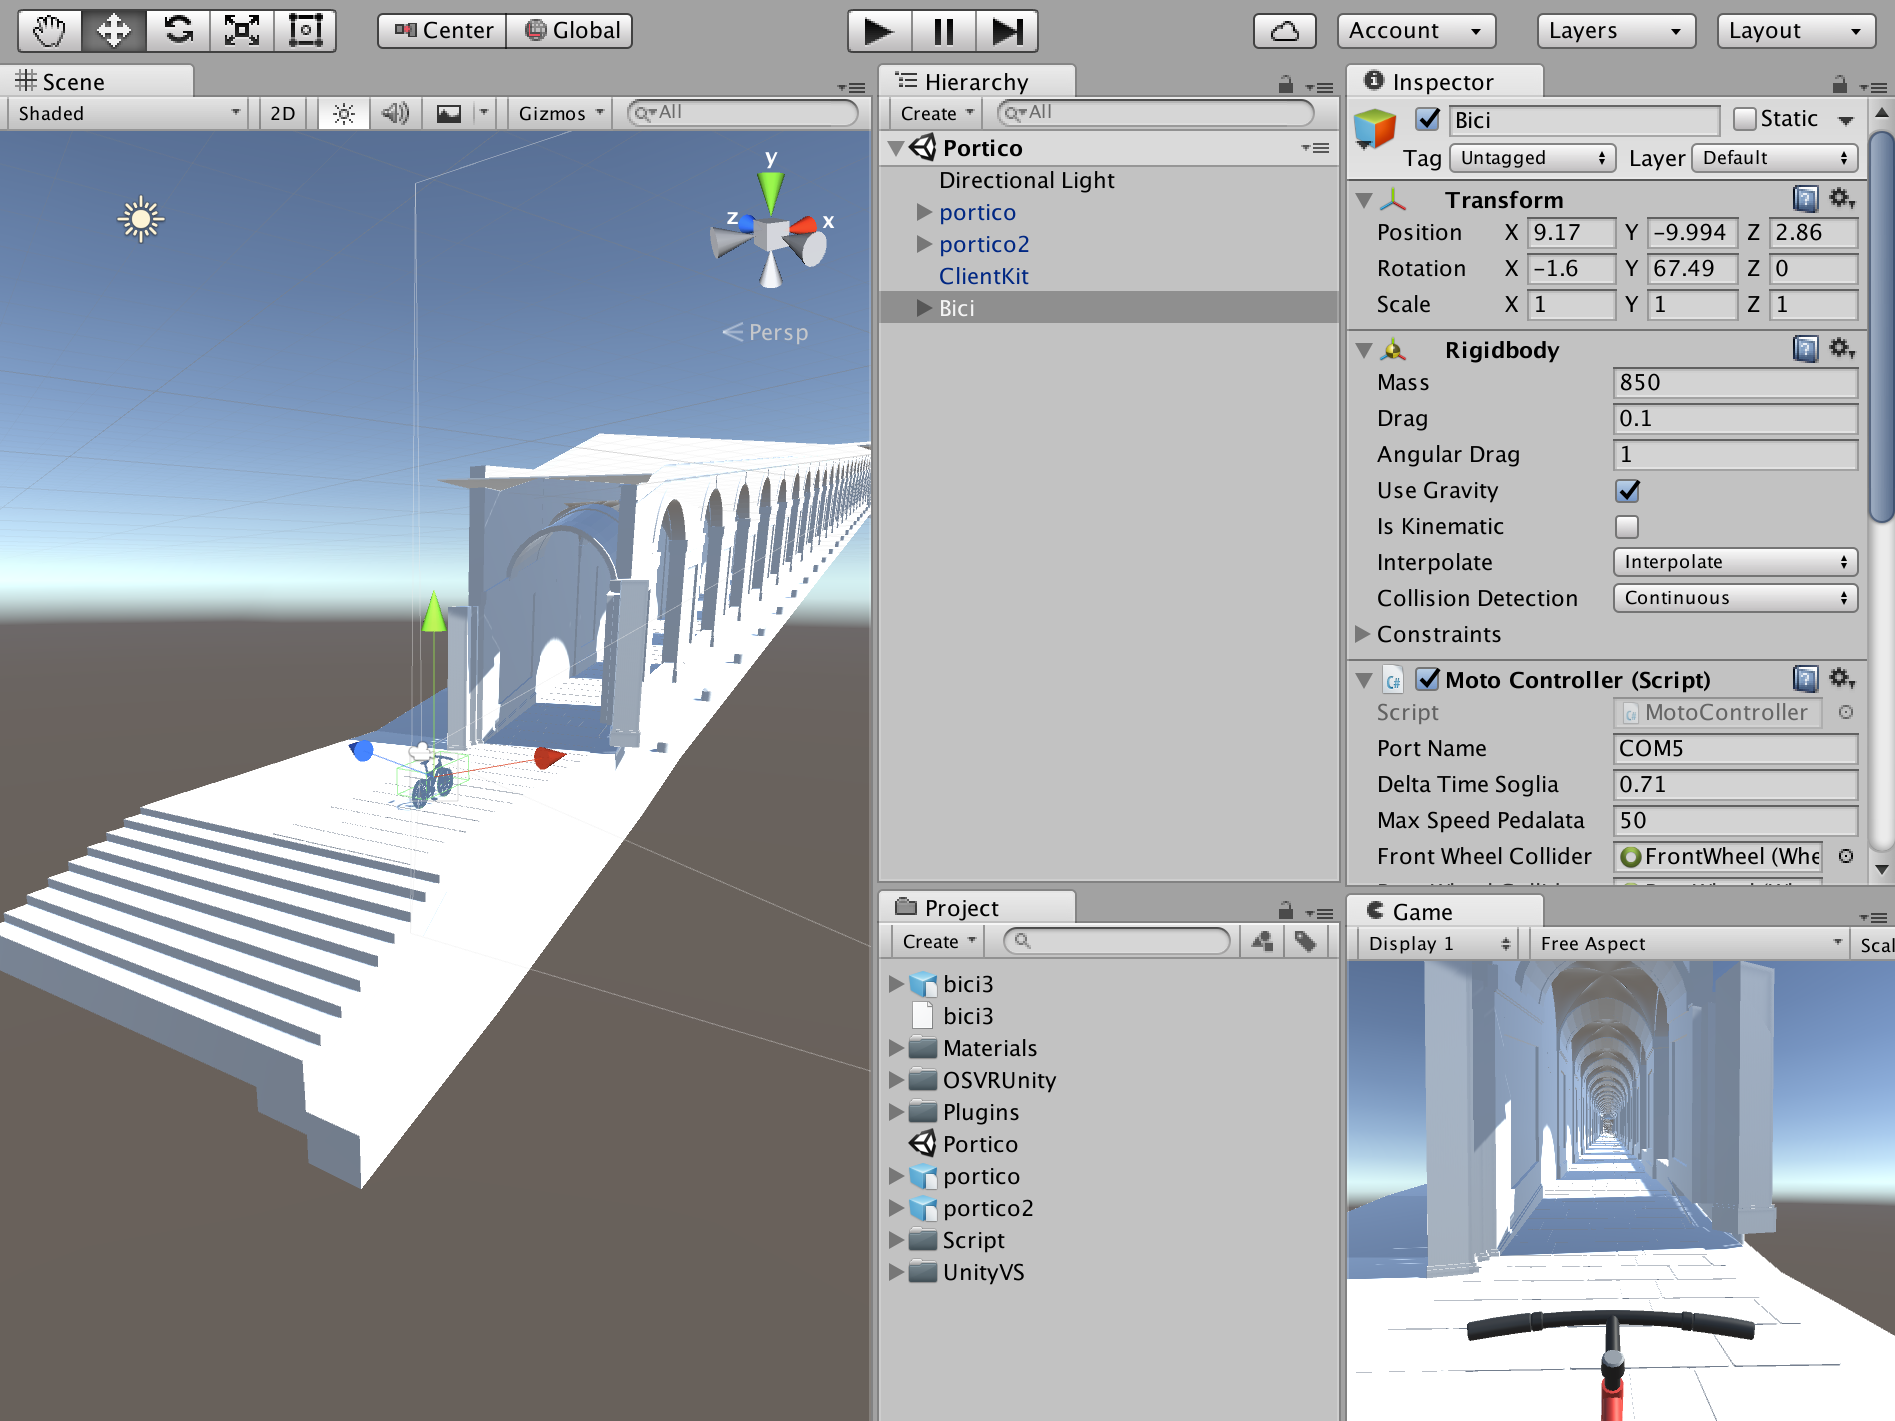
\includegraphics[width=\textwidth]{screenunity}
    \caption{La schermata principale di Unity\label{fig:screenunity}}
    \vspace{-0.3cm}
\end{figure}

\begin{itemize}
  \item \textbf{Scene}: dove viene mostrata l'architettura dell'ambientazione e degli oggetti. All'interno di quest'area si ha la possibilità di modificare gli oggetti, scalarli, muoverli e/o ruotarli. È inoltre possibile cambiare visualizzazione e vista utilizzando mouse e tastiera.
 \item \textbf{Game}: in questo riquadro è possibile osservare l'inquadratura della telecamera o del visore quando la simulazione è avviata. È inoltre possibile interagire con tastiera per muovere gli oggetti o spostare la visuale.
  \item \textbf{Inspector}: questo pannello permette allo sviluppatore di modificare tutti i valori relativo ad un oggetto selezionato. Permette inoltre di assegnare script che modellino a tempo di esecuzione l'oggetto, come ad esempio modificandone la posizione e/o creando animazioni per muoverlo. 
  \item \textbf{Hierarchy}: in questo punto sono elencati tutti gli oggetti presenti nella scena in ordine di parentela o di directory. Ogni componente può averne al suo interno altre (figlie) e può essere usata per trasferire delle caratteristiche quali la posizione, la rotazione e/o vincolare quest'ultime ai comportamenti del padre. Grazie al pulsante Create si possono aggiungere nuovi elementi alla scena. Ogni elemento aggiunto può essere messo in gerarchia semplicemente trascinandolo su un altro con il mouse, questi possono essere oggetti 2D e 3D, telecamere, luci, ecc.
    \item \textbf{Project}: in questa sezione è possibile rintracciare tutte le cartelle e i file del progetto. Questa sezione può interagire con Hierarchy: è infatti possibile trascinare oggetti prefabbricati (come ad esempio la bicicletta creata in Blender) e posizionarli nella scena.
\end{itemize}
Ogni oggetto che fa parte del progetto è elencato all’interno del riquadro Project ed ogni oggetto che fa parte della scena si può trovare all’interno di Hierarchy. Gli oggetti all’interno di Hierarchy vengono chiamati GameObject e ognuno di questi può essere salvato come componente Prefab, con tutti i suoi figli, e riutilizzato in tutte le scene come oggetto identicamente uguale al GameObject che lo ha originato. Questa funzione risulta utile nel caso servano istanze multiple dello stesso GameObject all’interno di una o più scene. Quando viene modificato il GameObject originario, le variazioni si propagano a tutte le sue istanze nel programma. Selezionando un GameObject da Hierarchy o anche dalla sezione Project la finestra Inspector si adatta alla caratteristiche in esso contenute. Ogni GameObject possiede al suo interno dei Component che ne definiscono caratteristiche e comportamento.

\subsubsection{Scenario Principale}
Durante la progettazione sono stati eseguiti due test diversi su due scenari diversi. Il primo test è stato eseguito nel modello dei portici di San Luca e serviva per testare il comportamento della bicicletta, in relazione alla fisica dell'attrito e dell'inerzia. Il motivo di questa scelta è dovuto alla pendenza dei portici, che portano la bicicletta a discendere per la gravità. Il secondo test è invece stato eseguito in un modello di Time Square, per verificare l'efficenza della pedalata, la velocità e la pendenza della bicicletta durante una sterzata. Tutte le calibrazioni riguardanti la fisica si tratteranno nella sezione \textit{\nameref{capitolo4}}. In questa sezione si descriverà lo scenario creato inizialmente per testare gli script che modellano il movimento della bicicletta a tempo di esecuzione. Il modello dei portici di San Luca è stato fornito diviso in 2 parti

\subsection{Motocontroller script}
spieghi ogni singolo comportamento dello scirpt
\subsection{ThreadDTWSlideWindow script}
spieghi ogni singolo comportamento dello scirpt




%
